%!TEX program = xelatex
\documentclass[11pt,a4paper]{article}
\usepackage[utf8]{inputenc}
\usepackage[T1]{fontenc}
\usepackage{ctex}
\usepackage{authblk}
\usepackage{tikz}
\usepackage{pgfplots}
\usepackage{verbatim}
\usepackage{amsfonts}
\usepackage{amsmath}
\usepackage{amsthm}
\usepackage{indentfirst}
\usepackage{amssymb}
\setlength{\parindent}{0pt}
\usetikzlibrary{shapes,snakes}
\newcommand{\argmax}{\operatornamewithlimits{argmax}}
\newcommand{\argmin}{\operatornamewithlimits{argmin}}

\DeclareMathOperator{\col}{col}
\usepackage{booktabs}
\newtheorem{theorem}{Theorem}
\newtheorem{proposition}{Proposition}
\newtheorem{lemma}{Lemma}
\newtheorem{example}{Example}
\newtheorem{corollary}{Corollary}
\newtheorem{note}{Note}
\usepackage{graphicx}
\usepackage{geometry}
\usepackage{hyperref}
\newcommand{\code}{	exttt}
\geometry{a4paper,scale=0.8}
\title{Linear Algebra}
\author[*]{Wenxiao Yang}
\affil[*]{Department of Mathematics, University of Illinois at Urbana-Champaign}
\date{2021}





\begin{document}
\maketitle
\tableofcontents
\newpage

\section{Vector Space}
\subsection{Vector Space $(V,+,\times)$ (over a field $\mathbb{F}$)}
A \underline{vector space} over a field $\mathbb{F}$ is a
set $V$ w/ an operation \underline{addition} $+ : V \times V \rightarrow V$ and
an operation \underline{scalar multiplication} $\mathbb{F} \times V \rightarrow V$\\
(1) Addition is associative $\&$ commutative\\
(2) $\exists 0\in V$, additive identity: $0 + v = v \forall v \in V$\\
(3) $1v = v \forall v \in V$(where $1 \in \mathbb{F}$ is multi. id. in $\mathbb{F}$ )\\
(4) $\forall \alpha,\beta\in\mathbb{F},\ v\in V,\ \alpha(\beta v)=(\alpha\beta)v$\\
(5) $\forall v\in V,\ (-1)v=-v$ we have $v+(-v)=0$\\
(6) $\forall \alpha\in\mathbb{F},\ v,u\in V,\ \alpha(v+u)=\alpha v+\alpha u$\\
(7) $\forall \alpha,\beta\in\mathbb{F},\ v\in V,\ (\alpha+\beta)v=\alpha v+\beta v$

\subsection{A field is a vector space over its subfield}
\begin{example}
$\mathbb{K}\subset\mathbb{F}$ is a subfield of a field $\mathbb{F}$. Then $\mathbb{F}$ is a vector space over $\mathbb{K}$. (Since $\mathbb{F}\subset \mathbb{F}[x]$, then $\mathbb{F}[x]$ is a vector space over $\mathbb{F}$.)
\end{example}
\subsection{ Vector subspace}
Suppose that $V$ is a vector space over $\mathbb{F}$. A \underline{vector subspace} or just \underline{subspace} is a nonempty subset $W\subset V$ closed under addition and scalar multiplication. i.e. $v+w\in W,\ av\in W,\ \forall v,w\in W,\ a\in \mathbb{F}$.\\
\begin{example}
$\mathbb{K}\subset \mathbb{L}\subset \mathbb{F}$, then $\mathbb{L}$ is a subspace of $\mathbb{F}$ over $\mathbb{K}$.
\end{example}
\subsection{Linear independent, Linear combination}
\subsection{span V, basis, dimension}
A set of elements $v_1,...,v_n\in V$ is said to \textbf{span} $V$ if every vector $v\in V$ can be expressed as a linear combination of $v_1,...,v_n$. If $v_1,...,v_n$ spans and is linearly independent, then we call the set a \textbf{\textit{basis}} for $V$.
\begin{proposition}[Proposition 2.4.10.]
    Suppose $V$ is a vector space over a field $\mathbb{F}$ having a basis $\{v_1,...,v_n\}$ with $n \geq 1$.
\end{proposition}
(i) For all $v \in V$ , $v = a_1 v_1 + ... + a_n v_n$ for exactly one $(a_1,...,a_n)\in \mathbb{F}^n$.\\
(ii) If $w_1,...,w_n$ span $V$ , then they are linearly independent.\\
(iii)If $w_1,...,w_n$ are linearly independent, then they span $V$.\\
If a vector space $V$ over $\mathbb{F}$ has a basis with $n$ vectors, then $V$ is said to be n-dimensional (over $\mathbb{F}$) or is said to have \textbf{dimension} $n$.
\subsection{Standard basis vectors}
\begin{equation}
    \begin{aligned}
        e_1=(1,0,...,0),e_2=(0,1,0,...,0),...,e_n=(0,0,...,0,1)\in \mathbb{F}^n
    \end{aligned}
    \nonumber
\end{equation}
are a basis for $\mathbb{F}^n$ called the \textbf{standard basis vectors}.
\subsection{Linear transformation}
Given two vector spaces $V$ and $W$ over $\mathbb{F}$ a \textbf{linear transformation} is a function $T : V \rightarrow	 W$ such that
for all $a \in \mathbb{F}$ and $v,w \in V$ , we have
\begin{equation}
    \begin{aligned}
        T(av)=aT(v)\ and\ T(v+w)=T(v)+T(w)
    \end{aligned}
    \nonumber
\end{equation}
\begin{proposition}[Proposition 2.4.15.]
    If $V$ and $W$ are vector spaces and $v_1,...,v_n$ is a basis for $V$ then any function
    from $\{v_1,...,v_n\}\rightarrow W$ extends \textit{uniquely} to a linear transformation $V \rightarrow W$.
\end{proposition}
Any $v\in V$, $\exists (a_1,...,a_n)$ s.t. $v=a_1 v_1+...+a_n v_n$. Then $T(v)=T(a_1 v_1+...+a_n v_n)=a_1T(v_1)+...+a_nT(v_n)$\\
\subsection{一个线性变换对应一个矩阵, 线性变换矩阵相乘仍为线性变换矩阵}
\begin{corollary}[Corollary 2.4.16.]
    If $v_1,...,v_n$ is a basis for a vector space $V$ and $w_1,...,w_n$ is a basis for a vector space $W$ (both over $\mathbb{F}$), then any linear transformation $T : V \rightarrow W$ determines (and is determined by) the $m\times n$ matrix:
    \begin{equation}
        \begin{aligned}
            A=A(T)=\begin{bmatrix}
                A_{11}&	A_{12}&... &A_{1n}\\
                A_{21}&	A_{22}&... &A_{2n}\\
                \vdots&	\vdots&... &\vdots\\
                A_{m1}&	A_{m2}&... &A_{mn}
            \end{bmatrix}
        \end{aligned}
        \nonumber
    \end{equation}
\end{corollary}
\begin{equation}
    \begin{aligned}
        &\begin{bmatrix}
            w_1&\cdots	&w_m
        \end{bmatrix}^T=A
        &\begin{bmatrix}
                v_1&\cdots	&v_n
        \end{bmatrix}^T
    \end{aligned}
    \nonumber
\end{equation}
$\mathcal{L} (V,M)$ denotes the set of all linear transformations from $V$ to $W$; $M_{m\times n}(\mathbb{F})$ the set of $m\times n$ matrix with entries in $\mathbb{F}$. $T\rightarrow A(T)$ defines a \textit{bijection} $\mathcal{L} (V,M)\rightarrow M_{m\times n}(\mathbb{F})$. \textbf{$A(T)$ represents the linear transformation $T$}.


\begin{proposition}[Proposition 2.4.19]
    Suppose that $V$ , $W$, and $U$ are vector spaces over $\mathbb{F}$, with fixed chosen bases. If
    $T : V \rightarrow W$ and $S : W \rightarrow U$ are linear transformations represented by matrices $A = A(T)$ and $B = B(S)$,
    then $ST = S \circ T : V \rightarrow U$ is a linear transformation represented by the matrix $BA = B(S)A(T)$.
\end{proposition}

\subsection{GL(V): invertible linear transformations $V \rightarrow	V$}
Given a vector space $V$ over $F$, we let $GL(V ) \subset \mathcal{L}(V , V )$ denote the subset of \textbf{invertible linear transformations}.
\begin{equation}
    \begin{aligned}
        GL(V)=\{T\in \mathcal{L}(V , V )| T \textit{ is a bijection}\}=\mathcal{L}(V , V )\cap Sym(V)
    \end{aligned}
    \nonumber
\end{equation}

\section{Euclidean geometry basics}
\subsection{Norm}
\subsubsection{Vector's Norm}
Vector $x \in \mathbb{R}^{n}$-n-dim Euclidean space
$$
x=\left(x_{1}, \ldots, x_{n}\right) \equiv\left[\begin{array}{llll}
x_{1} & x_{2} & \ldots & x_{n}
\end{array}\right]^{\top}=\left[\begin{array}{c}
x_{1} \\
x_{2} \\
\vdots \\
x_{n}
\end{array}\right]
$$

Norm of $x$, $\|x\|$ satisfies properties:

$$
\begin{aligned}
&\text { (a) }\|x\| \geqslant 0 \\
&\text { (b) }\|x\|=0 \Leftrightarrow x=0 \\
&\text { (c) }\|c x\|=|c|\|x\| \text {, for } c \in \mathbb{R} \\
&\text { (d) }\|x+y\| \leqslant\|x\|+\|y\| \longleftarrow \text { Triangle Ineq. }
\end{aligned}
$$

Enclidean Norm (default $\rho=2$): $\|x\|=\sqrt{x^{\top} x}=\sqrt{\sum_{i=1}^{n} x_{i}{ }^{2}}$

Other norms:

1. $l_{1}$-norm : $\|x\|_{1}=\sum_{i=1}^{n}\left|x_{i}\right|$

2. $l_{\rho}$-norm : $\|x\|_{\rho}=\sqrt[\rho]{\sum_{i=1}^{n}\left|x_{i}\right|^\rho}$

3. Supremum norm or $l_{\infty}$-norm : $\|x\|_{\infty}=\max _{i}\left|x_{i}\right|$

\subsubsection{Matrix's Norm}
$A\in \mathbb{R}^{n\times m}$ is a matrix

$\|A x\| \leqslant\|A\|\|x\|,\|A B\| \leqslant\|A\|\|B\|$

Default is $\rho=1$: $\|A\|=\max _{\|x\|=1}\|A x\|$. 即找到最大的绝对值和的“列”。

$\|A\|_{F}=\sqrt{\sum_{i, j} a_{i j}^{2}} \quad$ (Frobenius norm)

$\|A\|_{1}=\max _{j} \sum_{i=1}^{n}\left|A_{i j}\right| \quad[\Pi]$

$\|A\|_{\infty}=\max _{2} \sum_{j=1}^{n}\left|A_{i j}\right|[\square]$

$\|A\|_{2}=\max _{k} \sigma_{k}, \sigma_{k}$ is the singurai veruee of $A$

$\|A\|=\max \left(\frac{\|A \times\|}{\|\times\|}\right) \Rightarrow\|A\| \geqslant \frac{\|A \times\|}{\|\times\|}$

$\|A \times\| \leqslant\|A\|\|x\|$

\subsection{ Euclidean distance, inner product}
\textbf{Euclidean distance} on $\mathbb{R}^n$:
\begin{equation}
    \begin{aligned}
        |x-y|=\sqrt{(x_1-y_1)^2+...+(x_n-y_n)^2}
    \end{aligned}
    \nonumber
\end{equation}
\textbf{Euclidean inner product}:
\begin{equation}
    \begin{aligned}
        x\cdot y=x_1y_1+\cdots +x_ny_n=x^Ty
    \end{aligned}
    \nonumber
\end{equation}


Two important results for Euchidean norm:

1) Pythagorean Theorem: If $x^{\top} y=0$,
\[ \|x+y\|^{2}=\|x\|^{2}+\|y\|^{2} \]

2) Cauchy - Schwarz Inequality:

$$
\begin{aligned}
&\left|x^{\top} y\right| \leqslant\|x\|\|y\| \\
&"=" \text { iff } x=\alpha y \text { for some } \alpha \in \mathbb{R}
\end{aligned}
$$

\subsection{Isometry}
An \textbf{isometry} of $\mathbb{R}^n$ is a bijection $\varPhi :\mathbb{R}^n \rightarrow \mathbb{R}^n$ that preserves distance, which means,
\begin{equation}
    \begin{aligned}
        |\varPhi(x)-\varPhi(y)|=|x-y|,\ \forall x,y\in \mathbb{R}^n
    \end{aligned}
    \nonumber
\end{equation}
We use $Isom(\mathbb{R}^n)$ denotes the set of all isometries of $\mathbb{R}^n$,
\begin{equation}
    \begin{aligned}
        Isom(\mathbb{R}^n)=\{\varPhi:\mathbb{R}^n \rightarrow \mathbb{R}^n | |\varPhi(x)-\varPhi(y)|=|x-y|,\ \forall x,y\in \mathbb{R}^n\}
    \end{aligned}
    \nonumber
\end{equation}


\begin{proposition}
$\varPhi, \varPsi \in Isom(\mathbb{R}^n)$, then $\varPhi\circ\varPsi, \varPhi^{-1}\in Isom(\mathbb{R}^n)$
\end{proposition}
\begin{proof}
\quad\\
Since $\varPhi,\varPsi$ are bijections, so is $\varPhi\circ\varPsi$. Moreover,\\
\begin{equation}
    \begin{aligned}
        &|\varPhi\circ\varPsi(x)-\varPhi\circ\varPsi(y)|=|\varPhi(\varPsi(x))-\varPhi(\varPsi(y))|=|\varPsi(x)-\varPsi(y)|=|x-y|\\
    \end{aligned}
    \nonumber
\end{equation}
Since $id\in Isom (\mathbb{R}^n)$,
\begin{equation}
    \begin{aligned}
        |x-y|=|id(x)-id(y)|=|\varPhi\circ\varPhi^{-1}(x)-\varPhi\circ\varPhi^{-1}(y)|=|\varPhi^{-1}(x)-\varPhi^{-1}(y)|
    \end{aligned}
    \nonumber
\end{equation}
\end{proof}

\subsection{ Linear isometries i.e. orthogonal group}
There is a matrix $A\in GL(n,\mathbb{R})$ i.e. a \textit{invertible linear transofrmations} $T_A: \mathbb{R}^n \rightarrow \mathbb{R}^n$ is given by $T_A(v)=Av$.
\begin{equation}
    \begin{aligned}
        T_A(v)\cdot T_A(w)=(Av)\cdot(Aw)=(Av)^t(Aw)=v^tA^tAw
    \end{aligned}
    \nonumber
\end{equation}
\begin{equation}
    \begin{aligned}
        A^tA=I\Leftrightarrow T_A(v)\cdot T_A(w)=v\cdot \Leftrightarrow T_A\in Isom(\mathbb{R}^n)
    \end{aligned}
    \nonumber
\end{equation}
We define the all isometries in \textit{invertible linear transofrmations} $\mathbb{R}^n \rightarrow \mathbb{R}^n$ as \textbf{orthogonal group}
\begin{equation}
    \begin{aligned}
        O(n)=\{A\in GL(n,\mathbb{R})|A^tA=I \}\subset GL(n,\mathbb{R})
    \end{aligned}
    \nonumber
\end{equation}

\subsection{Special orthogonal group}
$O(n)$ are the matrices representing linear isometries of $\mathbb{R}^n$.
$1=det(I)=det(A^tA)=det(A^t)det(A)=det(A)^2 \Rightarrow	det(A)=1$ or $det(A)=-1$. We use \textbf{special orthogonal group} represents $A$ with $det(A)=1$,
\begin{equation}
    \begin{aligned}
        SO(n)=\{A\in O(n) | det(A)=1\}
    \end{aligned}
    \nonumber
\end{equation}

\subsection{translation}
Define a \textit{translation} by $v\in \mathbb{R}^n$,
\begin{equation}
    \begin{aligned}
        \tau_v:\mathbb{R}^n \rightarrow \mathbb{R}^n,\ \tau_v(x)=x+v
    \end{aligned}
    \nonumber
\end{equation}
\begin{note}[Exercise 2.5.3]
$\forall v\in \mathbb{R}^n, \tau_v$ is an isometry.
\end{note}
\begin{proof}
$|\tau_v(x)-\tau_v(y)|=|(x+v)-(y+v)|=|x-y|$
\end{proof}

\subsection{All isometries can be represented by a composition of \textit{a translation} and \textit{an orthogonal transformation}}
Since \textit{the composition of isometries is an isometry,} $\forall A\in O(n)$ and $v\in \mathbb{R}^n$, the composition
\begin{equation}
    \begin{aligned}
        \Phi_{A,v}(x)=\tau_v(T_A(x))=Ax+v
    \end{aligned}
    \nonumber
\end{equation}
is an isometry. \textbf{which could account for all isometries}.
\begin{theorem}
$Isom(\mathbb{R}^n)=\{\Phi_{A,v}|A\in O(n), v\in \mathbb{R}^n \}$
\end{theorem}

\section{Algebra Computation}
\subsection{ Random Vectors}
Mean:
$$\mu =\mathbb{E}(\mathbf{Z})=\begin{pmatrix}
    \mathbb{E}(Z_1)\\
    \mathbb{E}(Z_2)\\
    \cdots\\
    \mathbb{E}(Z_m)
\end{pmatrix}$$
Variance-Covariance matrix $\Sigma$:
$$\Sigma_{m\times m}=Cov(\mathbf{Z})=\mathbb{E}((\mathbf{Z}-\mu)(\mathbf{Z}-\mu)^T)=\begin{bmatrix}
    Var(Z_1)&\cdots	&Cov(Z_1,Z_m)\\
    \cdots&\cdots	&\cdots\\
    Cov(Z_m,Z_1)&\cdots &Var(Z_m)
\end{bmatrix}$$

Affine Transformation

(1)
$$\mathbf{W}=\mathbf{a}_{n\times 1}+\mathbf{B}_{n\times m}\mathbf{Z}_{m\times 1}$$
$$\mathbb{E}(\mathbf{W})=\mathbf{a}+\mathbf{B}\mu,\ Cov(\mathbf{W})=\mathbf{B}\Sigma \mathbf{B}^T$$
(2)
$$\mathbf{W}=\mathbf{v}^T \mathbf{Z}=v_1Z_1+...+v_mZ_m$$
$$\mathbb{E}(\mathbf{W})=\mathbf{v}^T\mu=\sum_{i=1}^mv_i\mu_i$$
$$Var(\mathbf{W})=\mathbf{v}^T\Sigma \mathbf{v}=\sum_{i=1}^mv_i^2Var(Z_i)+2\sum_{i<j}v_iv_jCov(Z_i,Z_j)$$
$$\text{i.e. }\mathbb{E}(\mathbf{A}\mathbf{Z})=\mathbf{A}\mathbb{E}(Z);\ Var(\mathbf{A}\mathbf{Z})=\mathbf{A}Var(\mathbf{Z})\mathbf{A}^T$$
(3)
$$Cov(\mathbf{A}\mathbf{X},\mathbf{B}\mathbf{Y})=\mathbb{E}[(\mathbf{A}\mathbf{X}-\mathbf{A}\mathbb{E}(X))(\mathbf{B}\mathbf{Y}-\mathbf{B}\mathbb{E}(Y))^T]=\mathbf{A}\mathbb{E}[(\mathbf{X}-\mathbb{E}(X))(\mathbf{Y}-\mathbb{E}(Y))^T]\mathbf{B}^T=\mathbf{A}Cov(\mathbf{X},\mathbf{Y})\mathbf{B}^T$$

\subsection{矩阵求导}
\href{https://zhuanlan.zhihu.com/p/24709748}{https://zhuanlan.zhihu.com/p/24709748}\\
\href{https://blog.csdn.net/daaikuaichuan/article/details/80620518}{https://blog.csdn.net/daaikuaichuan/article/details/80620518}

Vector by vector:
\begin{center}\begin{figure}[htbp]
    \centering
    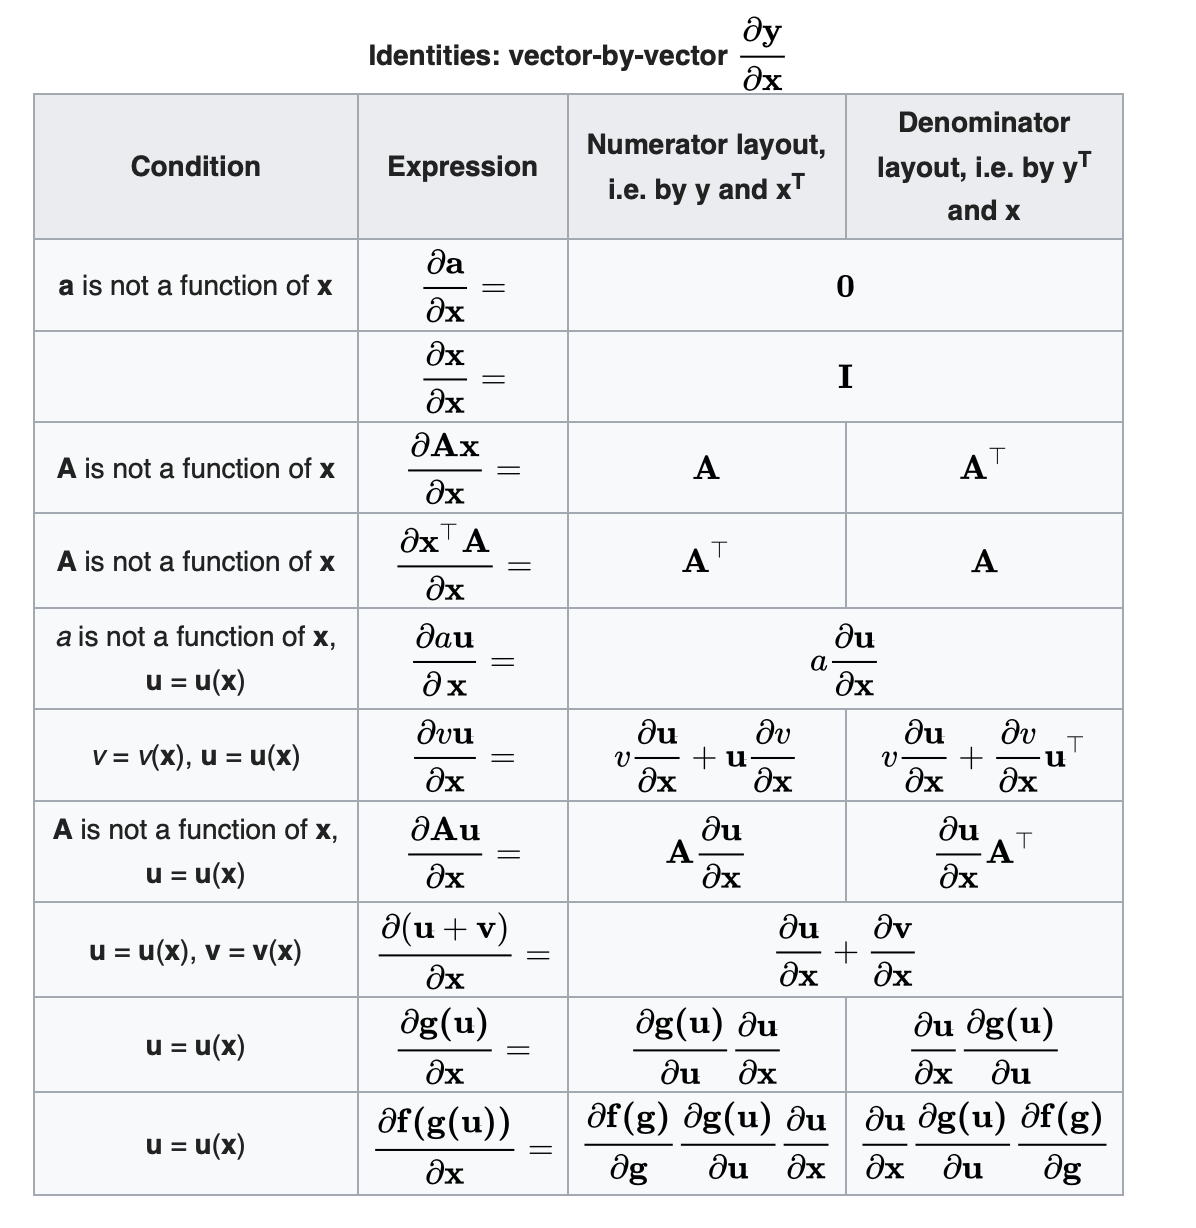
\includegraphics[scale=0.5]{vector_by_vector.png}
    \caption{}
    \label{}
\end{figure}\end{center}






















\begin{thebibliography}{1}
    \bibitem{Long2015Fully}  MATH 417: Christopher J Leininger  \newblock Introduction to Abstract Algebra (Draft)  2017.
    \bibitem{Long2015Fully} MATH 484
    \bibitem{Long2015Fully} ECE 490
    \bibitem{Long2015Fully} STAT 425
    \bibitem{Long2015Fully} CS/MATH 357
\end{thebibliography}


\end{document}
\bibliography{reference}
\bibliographystyle{unsrt}